\section{Introduction and Schedule Generation}
\subsection{The Problem}
\begin{frame}[fragile]{\insertsection}{\insertsubsection}
  \begin{itemize}
	\item Limited opportunities for communication 
	\item Human errors
	\item Ensure continued operation 
  \end{itemize}
\end{frame}

\begin{frame}[fragile]{Requirements}{\insertsubsection}
	\begin{itemize}
		\item Dependencies
		\item Windows
		\item Battery level
		\item Payload efficiency
	\end{itemize}
\end{frame}

\begin{frame}{Flow chart}{\insertsubsection}
	\begin{figure}
		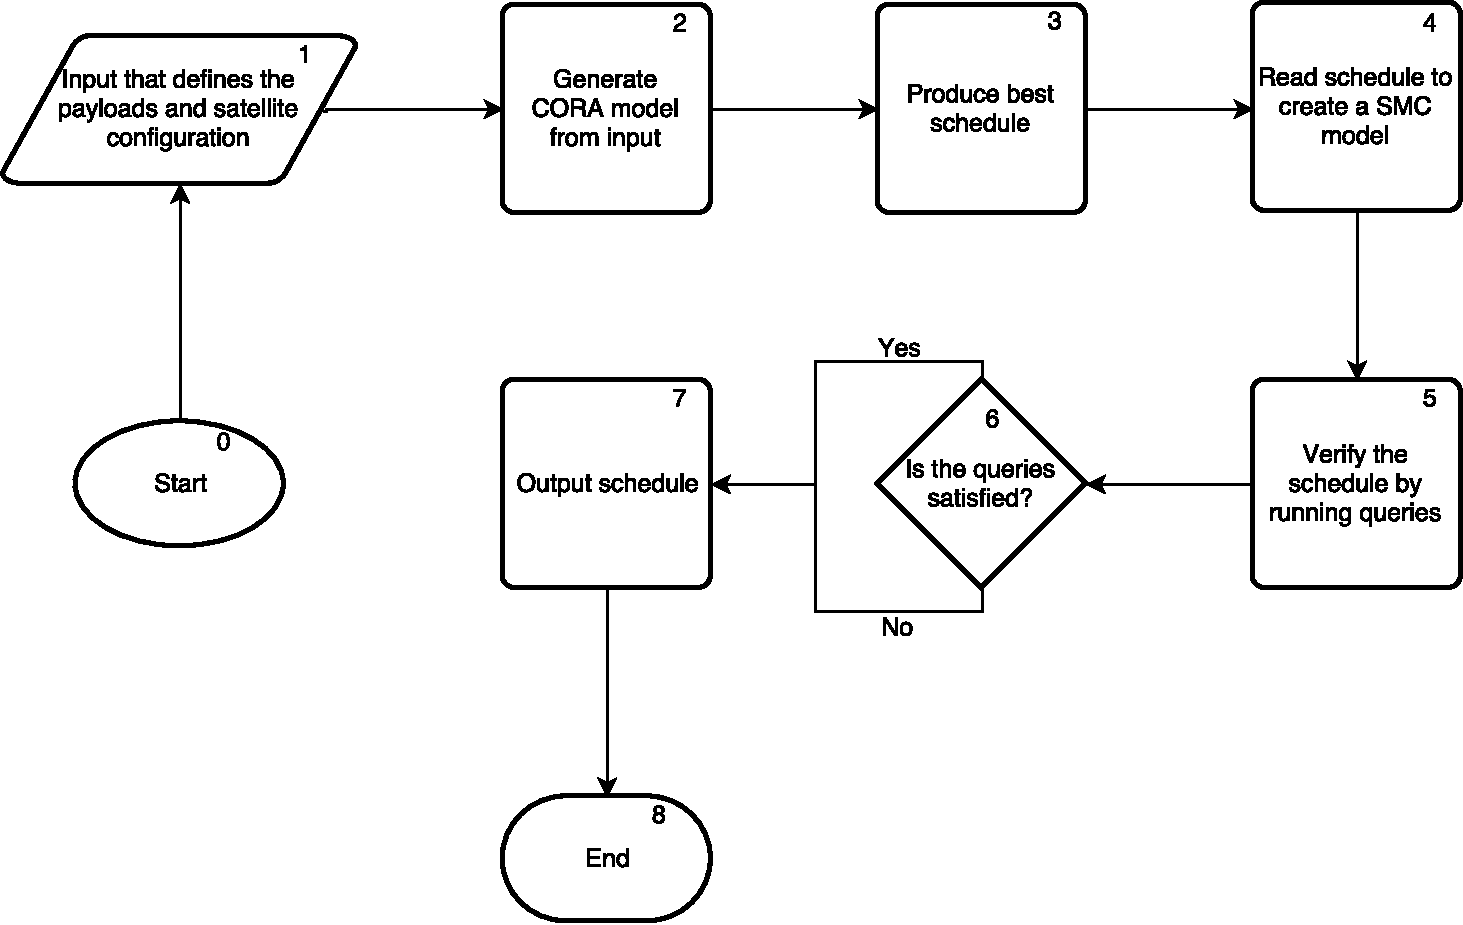
\includegraphics[width=.8\textwidth]{graphics/flow_final.pdf}
	\end{figure}
\end{frame}

\subsection{CORA Model}
\begin{frame}[fragile]{Schedule Generation}{Processor}
\begin{figure}
	\scalebox{.6}{
	\begin{tikzpicture}
	%Locations
	\node [init] (l0) {$\cup$};
	\node [location] (l1) [right of=l0, xshift=30mm] {$\cup$};
	\node [location] (l2) [right of=l1, xshift=40mm, label={
		[align=left]right:
		\textcolor{name}{ready}
	}] {$\cup$};
	\node [location] (l3) [below of=l1, yshift=-30mm, label={
		[align=right]left:
		\textcolor{name}{Wait}\\
		\textcolor{invariant}{x <= TaskTimes[active][2]}
	}] {};
	\node [location] (l4) [below of=l2, yshift=-30mm, label={
		[align=left]right:
		\textcolor{name}{running}\\
		\textcolor{invariant}{x <= TaskTimes[active][1]}\\
		\textcolor{invariant}{\&\& cost' == runCost}
	}] {};
	\node [location] (l5) [above of=l2, yshift=35mm] {C};
	\node [location] (l6) [above of=l1, yshift=35mm, label={
		[align=left]above:
		\textcolor{name}{Idle}\\
		\textcolor{invariant}{cost' == 5}
	}] {};
	\path[->,black, thick] (l0) edge node [midway, below ][align=center]{\textcolor{update}{mayRun()}} (l1);
	\path[->,black, thick] (l1) edge node [midway, above][align=left]{
		\textcolor{select}{a: int[0,N-1]}\\
		\textcolor{guard}{runnableCount() > 0}\\
		\textcolor{guard}{\&\& runnable[a] == 1}\\
		\textcolor{sync}{ready!}\\
		\textcolor{update}{mayRun(), active = a}} (l2);
	\path[->,black, thick] (l2) edge node [midway, right][align=left]{
		\textcolor{guard}{runnable[active] == 1}\\
		\textcolor{guard}{\&\& !checkBattery()}\\		
		\textcolor{sync}{run?}\\
		\textcolor{update}{updateBattery(), calcCost()}} (l4);
	\path[->,black, thick] (l2) edge[bend right=35] node [midway, left][align=center]{
		\textcolor{sync}{run?}}(l6);
	\path[->,black, thick] (l4) edge node [midway, below][align=center]{
		\textcolor{guard}{x >= TaskTimes[active][1]}} (l3);
	\path[->,black, thick] (l3) edge node [midway, left][align=right]{
		\textcolor{guard}{x >= TaskTimes[active][2]}\\
		\textcolor{update}{reset(), dequeue(),}\\
		\textcolor{update}{x = 0, mayRun()}} (l1);
	\path[->,black, thick] (l1) edge node [midway, left][align=left]{
		\textcolor{guard}{runnableCount() == 0}} (l6);
	\path[->,black, thick] (l6) edge node [midway, above][align=left]{
		\textcolor{sync}{win?}} (l5);
	\path[->,black, thick] (l5) edge node [midway, right][align=left]{
		\textcolor{select}{a: int[0,N-1]}\\
		\textcolor{sync}{ready!}\\
		\textcolor{update}{mayRun(), active = a}} (l2);
	\path[->,black, thick] (l2) edge[bend left=45] node [midway, below][align=center]{
		\textcolor{guard}{runnable[active] == 0}\\
		\textcolor{guard}{\&\& !checkBattery()}\\
		\textcolor{sync}{run?}} (l1);
	\end{tikzpicture}
}
\end{figure}
\end{frame}

\begin{frame}[fragile]{Schedule Generation}{Scheduler}
\begin{figure}[H]
	\centering
	\scalebox{.9}{
	\begin{tikzpicture}
	%Locations
	\node [init] (l0) [label={[align=left]left:
		\textcolor{invariant}{checkBattery()}
	}] {};
	\node [location] (l1) [right of=l0, xshift=40mm, label={
		[align=left]right:
		\textcolor{invariant}{checkBattery()}
	}] {$\cup$};
	\path[->,black, thick] (l0) edge[bend left=30] node [midway, above][align=center]{
		\textcolor{sync}{ready?}} (l1);
	\path[->,black, thick] (l1) edge[bend left=30] node [midway, below][align=center]{
		\textcolor{sync}{run!}} (l0);
	\end{tikzpicture}
}
\end{figure}
\end{frame}

\begin{frame}[fragile]{Schedule Generation}{Processor}
	\begin{figure}
		\scalebox{.6}{
			\begin{tikzpicture}
			%Locations
			\node [init] (l0) {$\cup$};
			\node [location] (l1) [right of=l0, xshift=30mm] {$\cup$};
			\node [location] (l2) [right of=l1, xshift=40mm, label={
				[align=left]right:
				\textcolor{name}{ready}
			}] {$\cup$};
			\node [location] (l3) [below of=l1, yshift=-30mm, label={
				[align=right]left:
				\textcolor{name}{Wait}\\
				\textcolor{invariant}{x <= TaskTimes[active][2]}
			}] {};
			\node [location] (l4) [below of=l2, yshift=-30mm, label={
				[align=left]right:
				\textcolor{name}{running}\\
				\textcolor{invariant}{x <= TaskTimes[active][1]}\\
				\textcolor{invariant}{\&\& cost' == runCost}
			}] {};
			\node [location] (l5) [above of=l2, yshift=35mm] {C};
			\node [location] (l6) [above of=l1, yshift=35mm, label={
				[align=left]above:
				\textcolor{name}{Idle}\\
				\textcolor{invariant}{cost' == 5}
			}] {};
			\path[->,black, thick] (l0) edge node [midway, below ][align=center]{\textcolor{update}{mayRun()}} (l1);
			\path[->,black, thick] (l1) edge node [midway, above][align=left]{
				\textcolor{select}{a: int[0,N-1]}\\
				\textcolor{guard}{runnableCount() > 0}\\
				\textcolor{guard}{\&\& runnable[a] == 1}\\
				\textcolor{sync}{ready!}\\
				\textcolor{update}{mayRun(), active = a}} (l2);
			\path[->,black, thick] (l2) edge node [midway, right][align=left]{
				\textcolor{guard}{runnable[active] == 1}\\
				\textcolor{guard}{\&\& !checkBattery()}\\		
				\textcolor{sync}{run?}\\
				\textcolor{update}{updateBattery(), calcCost()}} (l4);
			\path[->,black, thick] (l2) edge[bend right=35] node [midway, left][align=center]{
				\textcolor{sync}{run?}}(l6);
			\path[->,black, thick] (l4) edge node [midway, below][align=center]{
				\textcolor{guard}{x >= TaskTimes[active][1]}} (l3);
			\path[->,black, thick] (l3) edge node [midway, left][align=right]{
				\textcolor{guard}{x >= TaskTimes[active][2]}\\
				\textcolor{update}{reset(), dequeue(),}\\
				\textcolor{update}{x = 0, mayRun()}} (l1);
			\path[->,black, thick] (l1) edge node [midway, left][align=left]{
				\textcolor{guard}{runnableCount() == 0}} (l6);
			\path[->,black, thick] (l6) edge node [midway, above][align=left]{
				\textcolor{sync}{win?}} (l5);
			\path[->,black, thick] (l5) edge node [midway, right][align=left]{
				\textcolor{select}{a: int[0,N-1]}\\
				\textcolor{sync}{ready!}\\
				\textcolor{update}{mayRun(), active = a}} (l2);
			\path[->,black, thick] (l2) edge[bend left=45] node [midway, below][align=center]{
				\textcolor{guard}{runnable[active] == 0}\\
				\textcolor{guard}{\&\& !checkBattery()}\\
				\textcolor{sync}{run?}} (l1);
			\end{tikzpicture}
		}
	\end{figure}
\end{frame}


\begin{frame}[fragile]{Schedule Generation}{Insolation}
\begin{figure}[H]
	\centering
	\scalebox{.6}{
	\begin{tikzpicture}
	%Locations
	\node [init] (l0) [label={
		[align=left]above:
		\textcolor{name}{inSun}
	}, label={
	[align=left]left:
	\textcolor{invariant}{splitTime <= OrbitTime / 8}\\
	\textcolor{invariant}{\&\& ins <= OrbitTime / 2}
}] {};
\node [location] (l1) [right of=l0, xshift=40mm, label={
	[align=left]above:
	\textcolor{name}{inEclipse}
}, label={
[align=left]right:
\textcolor{invariant}{splitTime <= OrbitTime / 8}\\
\textcolor{invariant}{\&\& ins <= OrbitTime / 2}
}] {};
%Edges
\path[->,black, thick] (l0) edge[bend left=30] node [midway, above][align=left]{
	\textcolor{guard}{ins >= OrbitTime / 2}\\
	\textcolor{guard}{\&\& chargeCount == 4}} (l1);
\path[->,black, thick] (l1) edge[bend left=30] node [midway, below][align=left]{
	\textcolor{guard}{ins >= OrbitTime}\\
	\textcolor{guard}{\&\& chargeCount == 8}\\
	\textcolor{update}{ins := 0,}\\
	\textcolor{update}{splitTime = 0}\\
	\textcolor{update}{chargeCount = 0}} (l0);
\path[->,black, thick] (l0) edge [loop below] node [midway, below left][align=left]{
	\textcolor{guard}{splitTime >= OrbitTime/8}\\
	\textcolor{update}{increaseBattery()}} (l0);
\path[->,black, thick] (l1) edge [loop below] node [midway, below right][align=left]{
	\textcolor{guard}{splitTime >= OrbitTime/8}\\
	\textcolor{update}{subIdle()}} (l1);
\end{tikzpicture}
}
\end{figure}
\end{frame}

\begin{frame}[fragile]{Schedule Generation}{Windows}
\begin{figure}[H]
	\centering
	\scalebox{.6}{
	\begin{tikzpicture}
	%Locations
	\node [init] (l0) {C};
	\node [location] (l1) [right of=l0, xshift=30mm, label={
		[align=center]above:
		\textcolor{name}{notIn}\\
		\textcolor{invariant}{wtime <= window[id][0]}
	}] {};
	\node [location] (l2) [right of=l1, xshift=45mm, label={
		[align=center]above:
		\textcolor{name}{in}\\
		\textcolor{invariant}{wtime <=}\\
		\textcolor{invariant}{window[id][1]}
	}] {};
	\node [location] (l3) [right of=l1, xshift=20mm, yshift=-60mm, label={
		[align=center]below:
		\textcolor{invariant}{wtime <= orbitTime}
	}] {};
	\node [location] (l4) [right of=l2, xshift=45mm]{C};
	\path[->,black, thick] (l0) edge node [midway, below][align=left]{
		\textcolor{update}{alwaysAvailable()}} (l1);
	\path[->,black, thick] (l1) edge node [midway, below][align=center]{
		\textcolor{guard}{wtime >= window[id][0]}\\
		\textcolor{update}{setRunnable()}\\
		\textcolor{sync}{win!}} (l2);
	\path[->,black, thick] (l3) edge node [midway, below left][align=right]{
		\textcolor{guard}{wtime >= orbitTime}\\
		\textcolor{update}{wtime = 0}\\
		\textcolor{sync}{win!}} (l1);
	\path[->,black, thick] (l2) edge node [midway, below right][align=left]{
		\textcolor{guard}{wtime >= window[id][1]}\\
		\textcolor{update}{removeRunnable()}\\
		\textcolor{sync}{win!}} (l3);
	\path[->,black, thick] (l2) edge node [midway, below][align=center]{
		\textcolor{sync}{ready?}} (l4);
	\path[->,black, thick] (l4) edge[bend left=30] node [midway, below][align=center]{
		\textcolor{guard}{ins+TaskTimes[active][1]}\\
		\textcolor{guard}{ >= Window[id][1]}\\
		\textcolor{update}{runnable[active] = 0}}(l2);
	\path[->,black, thick] (l4) edge[bend right=30] node [midway, above][align=center]{
		\textcolor{guard}{ins+TaskTimes[active][1]}\\
		\textcolor{guard}{<= Window[id][1]}}(l2);
	\end{tikzpicture}
}
\end{figure}
\end{frame}

